\chapter{Anhang}

\section{Spielstände}
\sectionauthor{\leonard}

\begin{figure}[h]
	\centering
	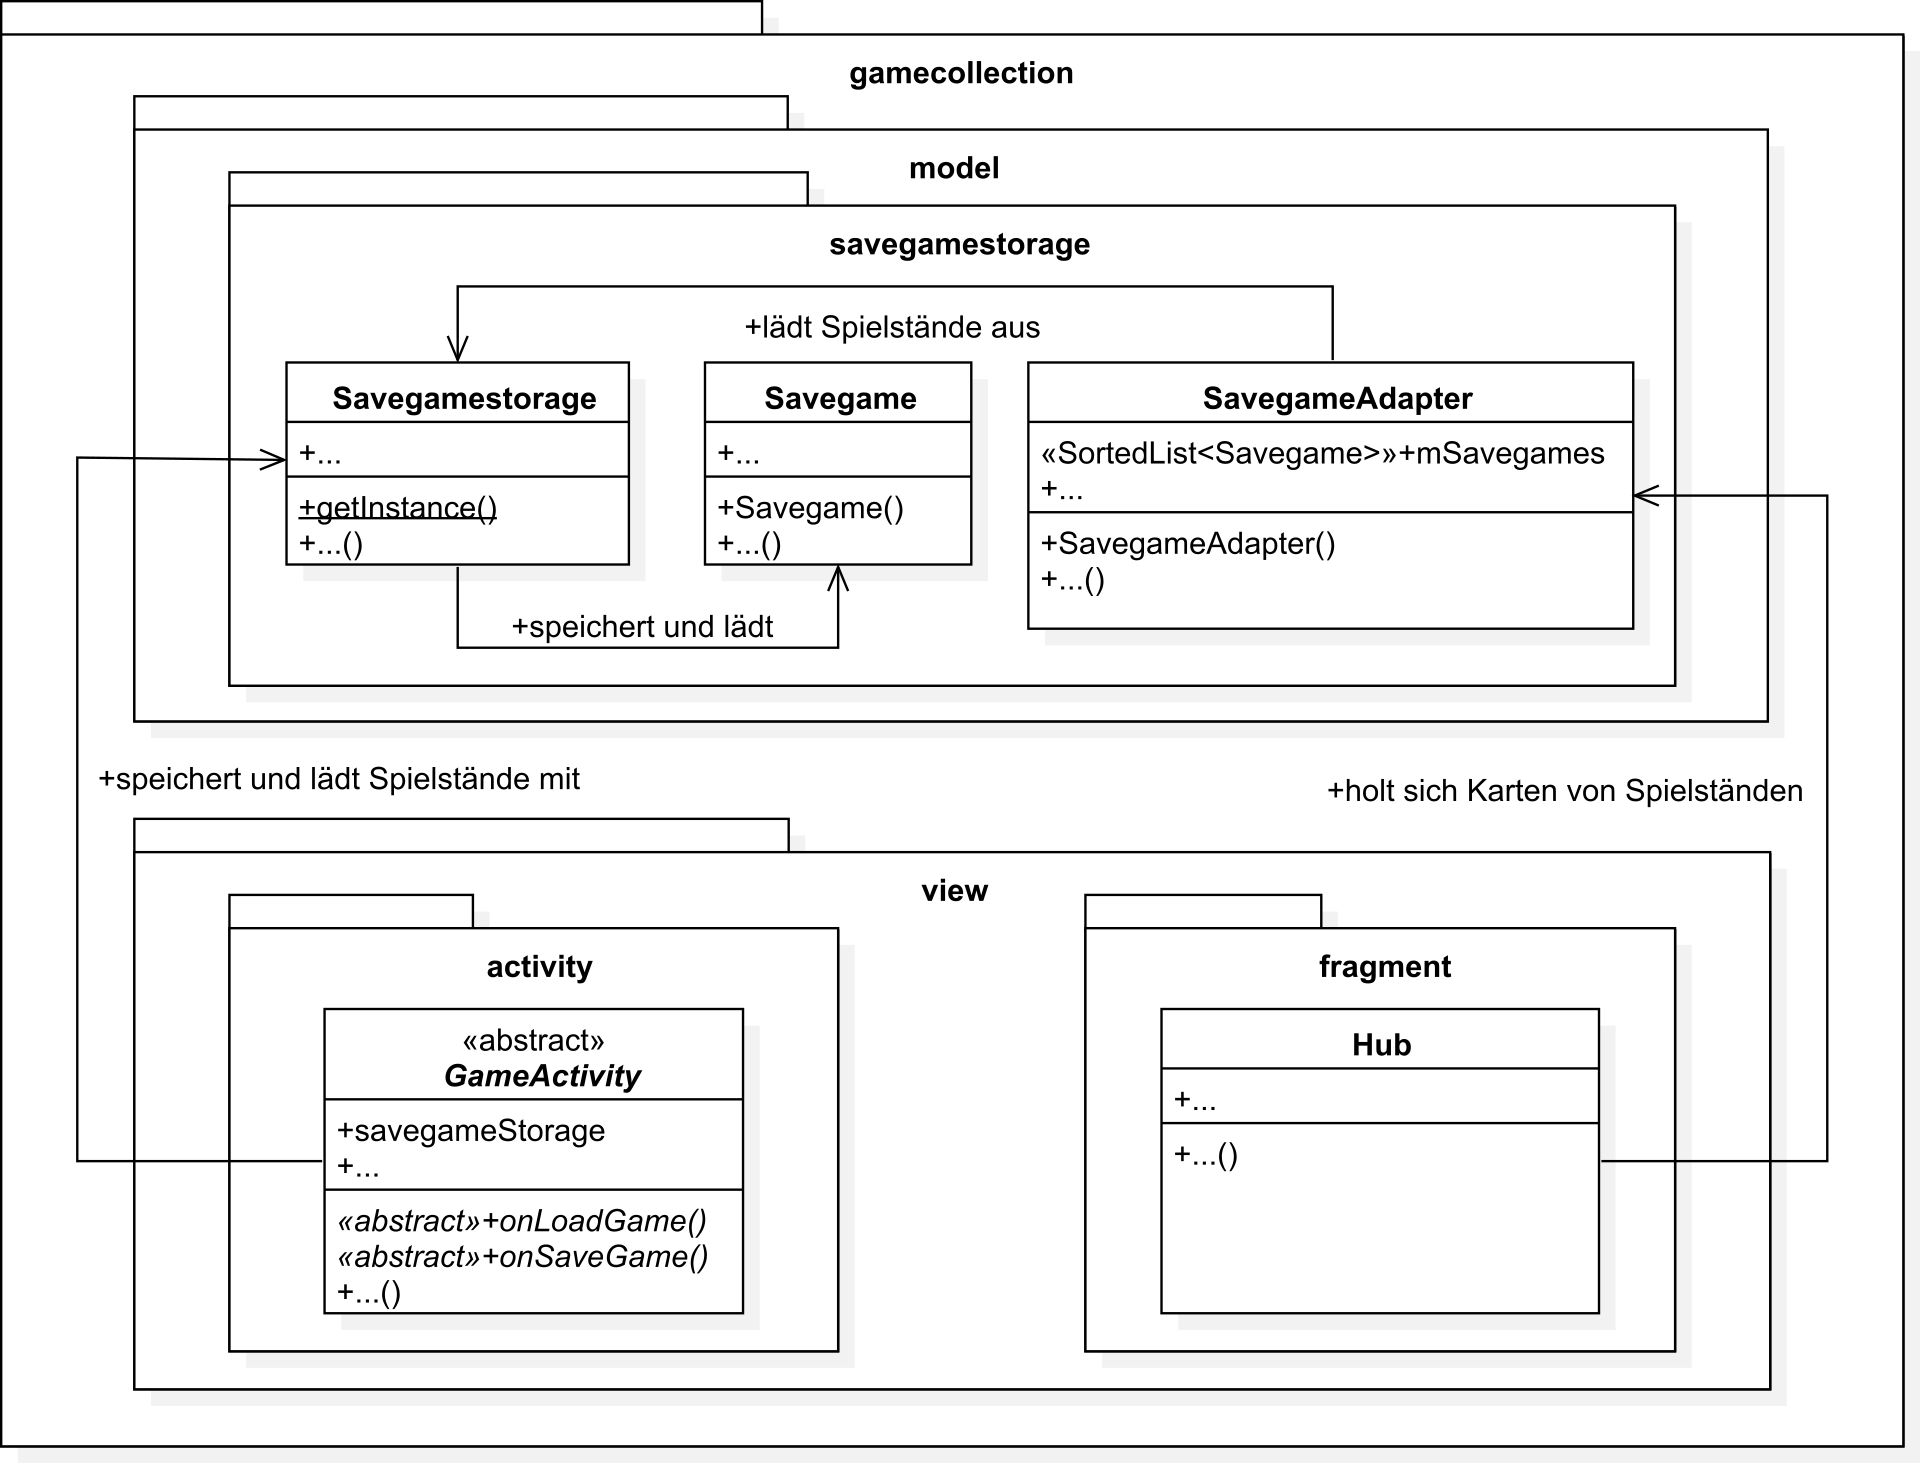
\includegraphics[width=1.0\textwidth]{resources/savegamestorage/Savegamestorage}
	\caption{Spielstand Architektur}
\end{figure}

\section{Schachevaluierung}

\begin{figure}[p]
\centering
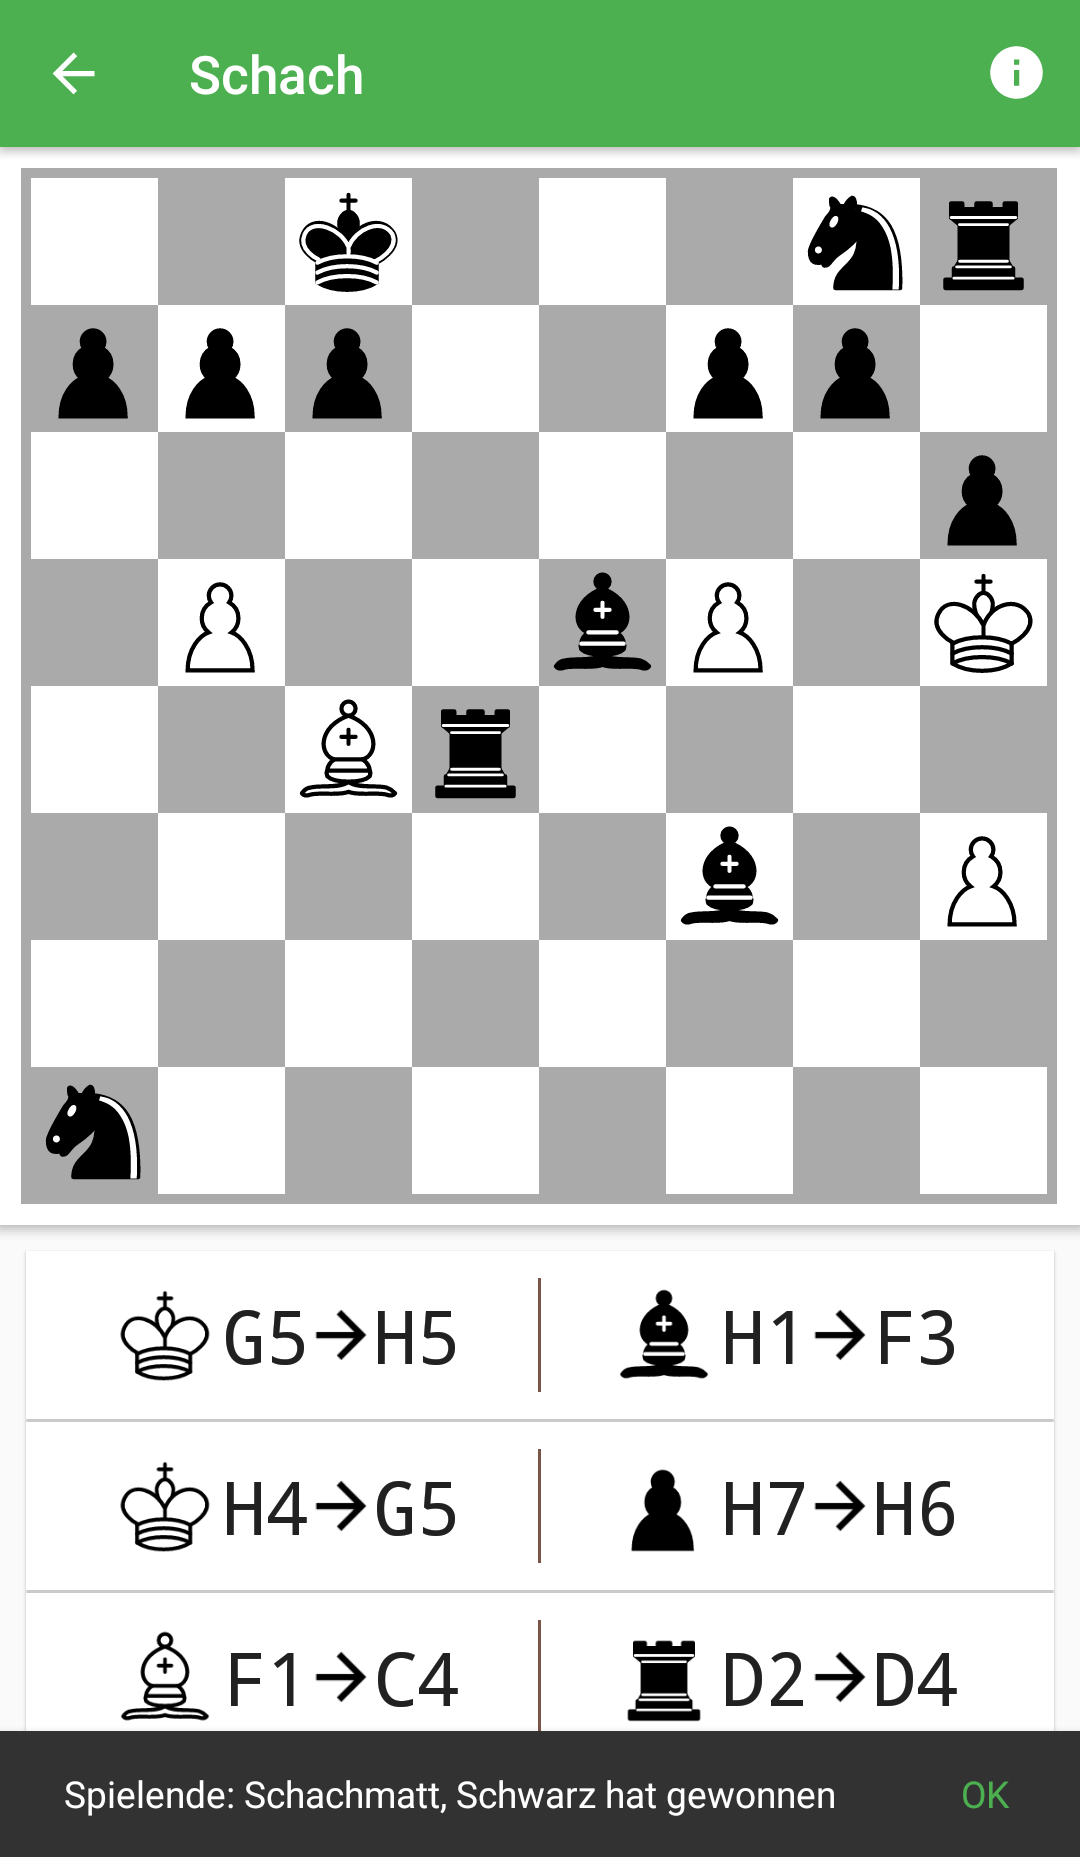
\includegraphics[width=.3\textwidth]{resources/evaluierung/chess/screen}
\caption{Evaluierung: Der Schachbildschirm}
\label{fig:screen}
\end{figure}

\begin{figure}[p]
\centering
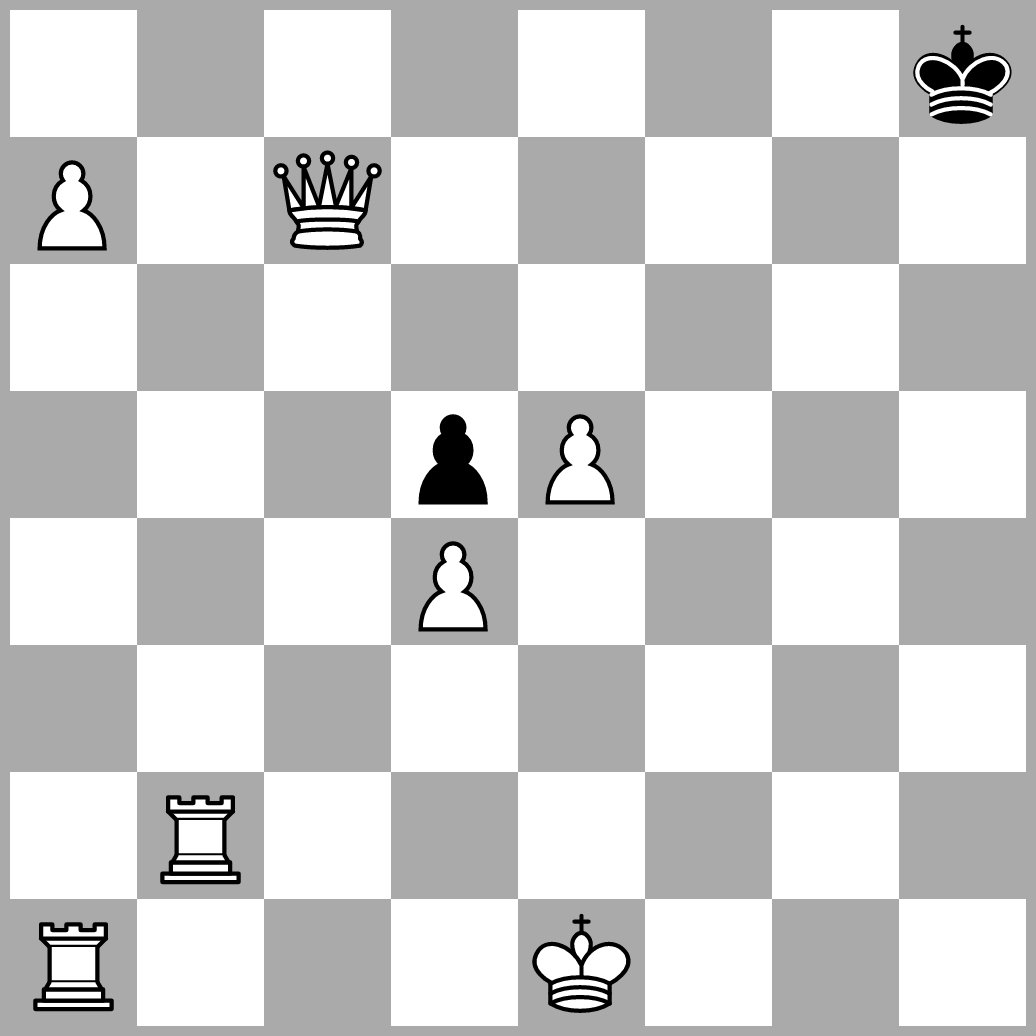
\includegraphics[width=.3\textwidth]{resources/evaluierung/chess/special}
\caption{Evaluierung: Aufstellung}
\label{fig:special}
\end{figure}

\begin{figure}[p]
\centering
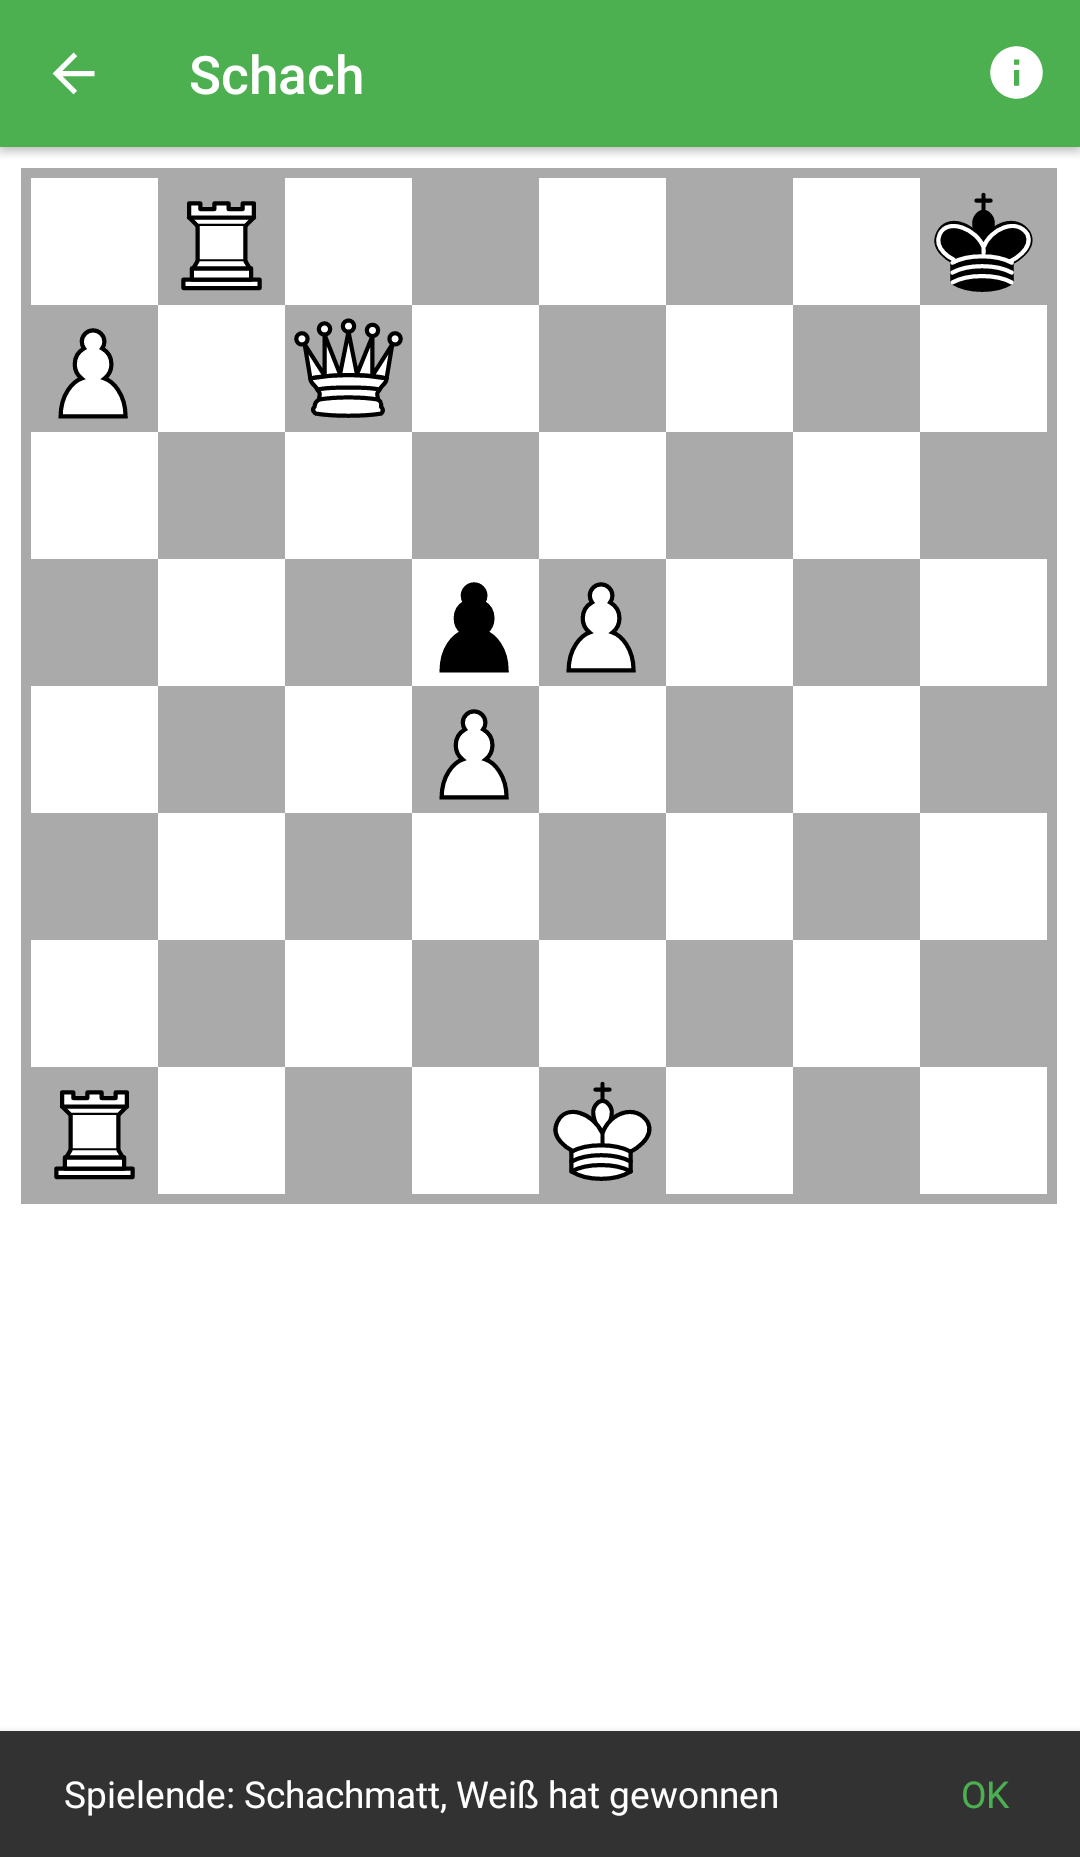
\includegraphics[width=.3\textwidth]{resources/evaluierung/chess/checkmate}
\caption{Evaluierung: Schachmatt}
\label{fig:checkmate}
\end{figure}

\begin{figure}[h]
\centering
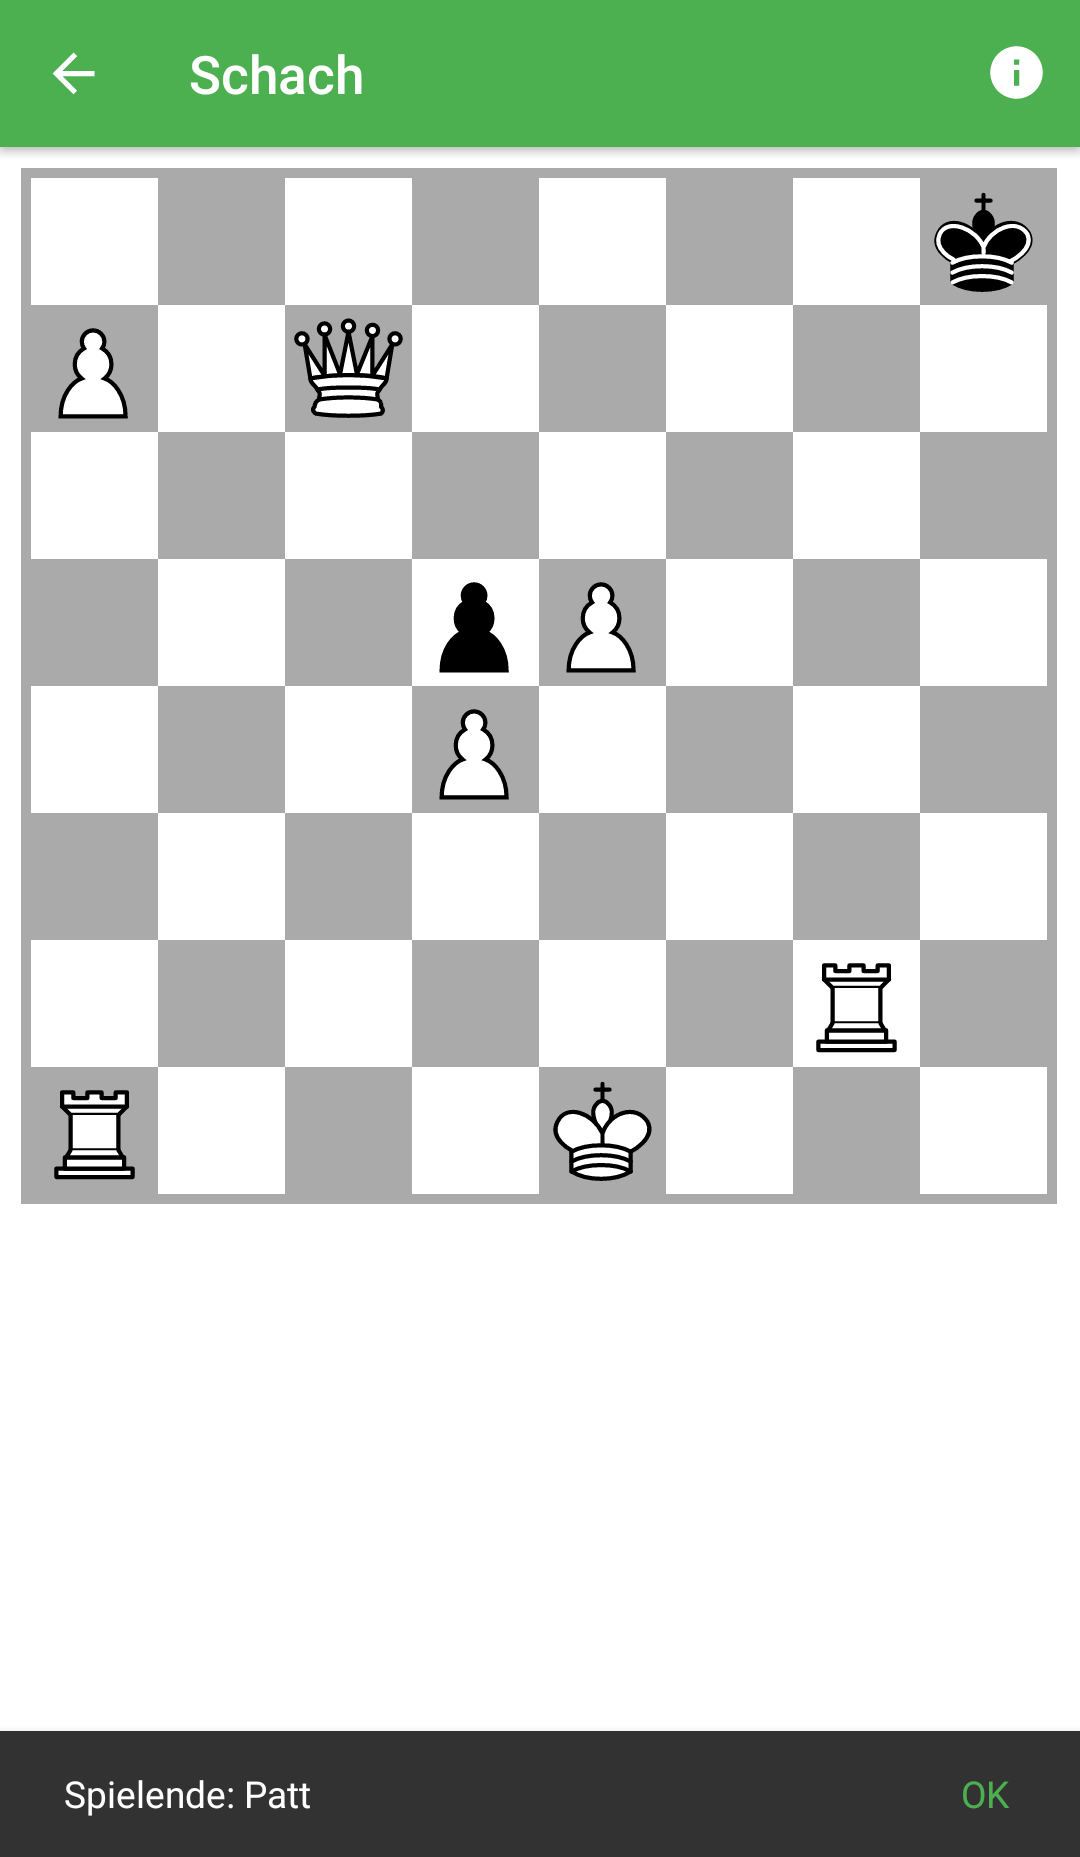
\includegraphics[width=.3\textwidth]{resources/evaluierung/chess/stalemate}
\caption{Evaluierung: Patt}
\label{fig:stalemate}
\end{figure}

\begin{figure}[h]
\centering
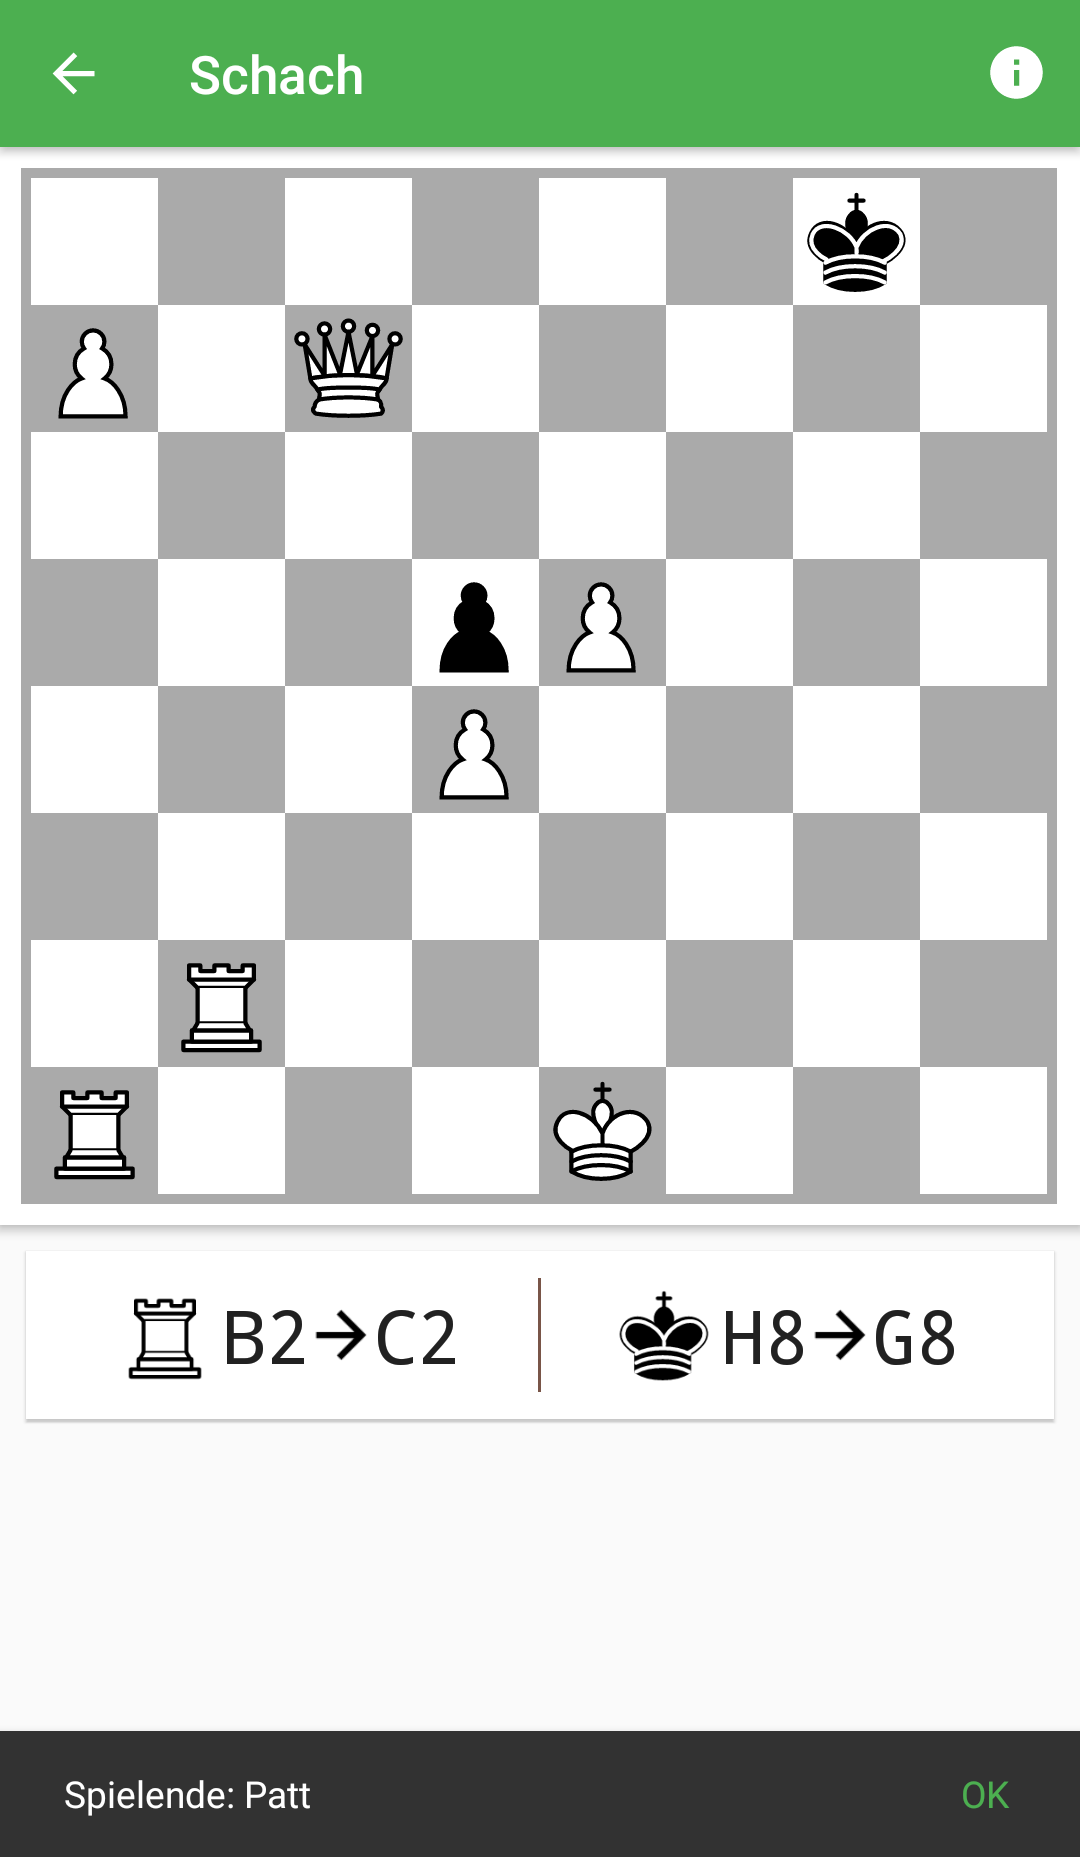
\includegraphics[width=.3\textwidth]{resources/evaluierung/chess/fifty_move}
\caption{Evaluierung: 50-Züge-Regel}
\label{fig:fifty_move}
\end{figure}

\begin{figure}[h]
\centering
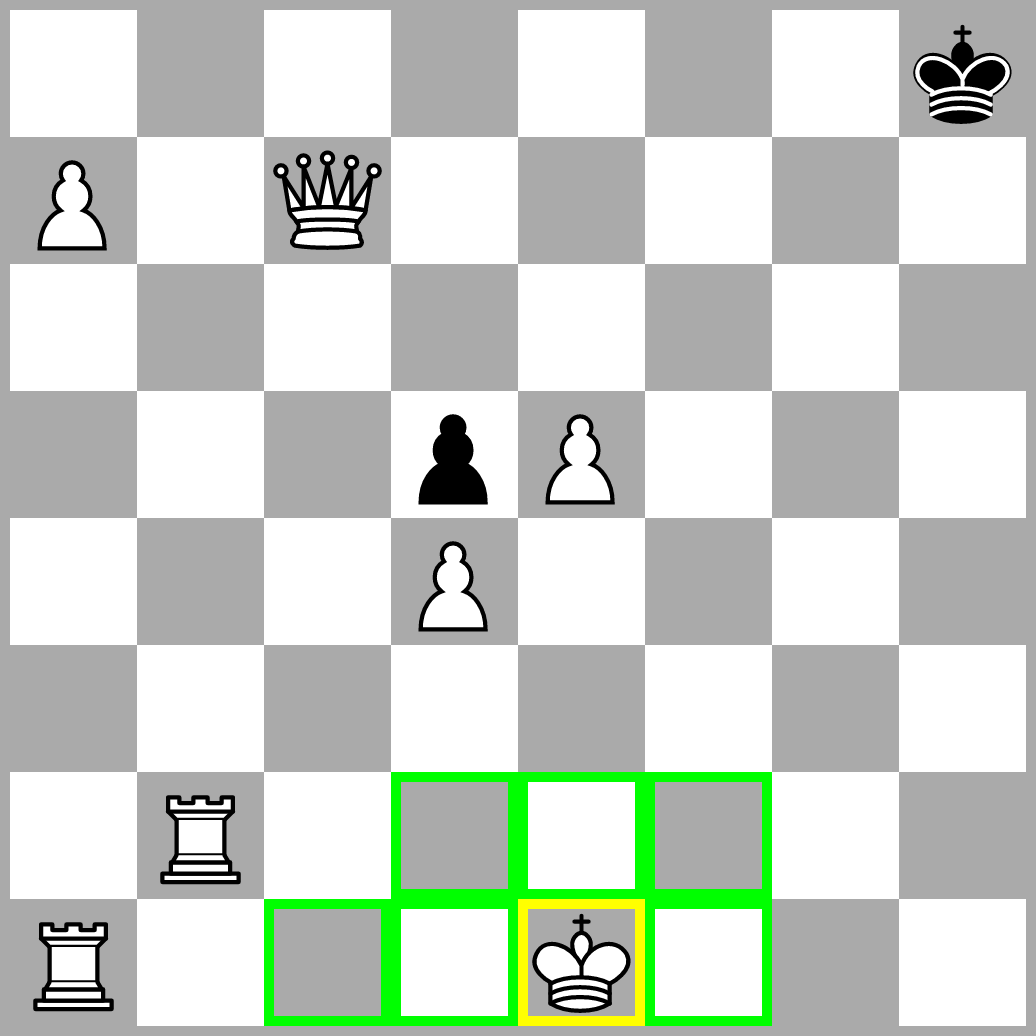
\includegraphics[width=.3\textwidth]{resources/evaluierung/chess/castling_before}
\caption{Evaluierung: Rochade vorher}
\label{fig:castling_before}
\end{figure}

\begin{figure}[h]
\centering
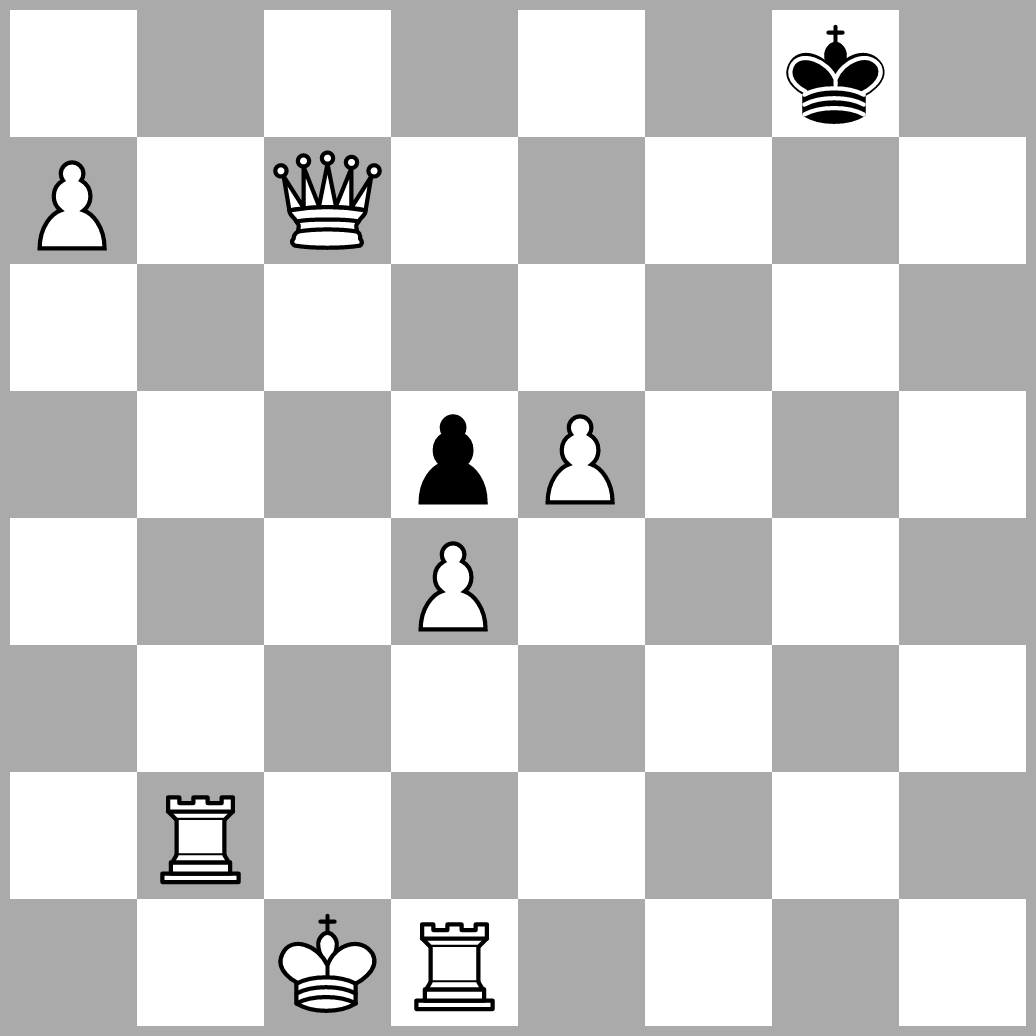
\includegraphics[width=.3\textwidth]{resources/evaluierung/chess/castling_after}
\caption{Evaluierung: Rochade danach}
\label{fig:castling_after}
\end{figure}

\begin{figure}[h]
\centering
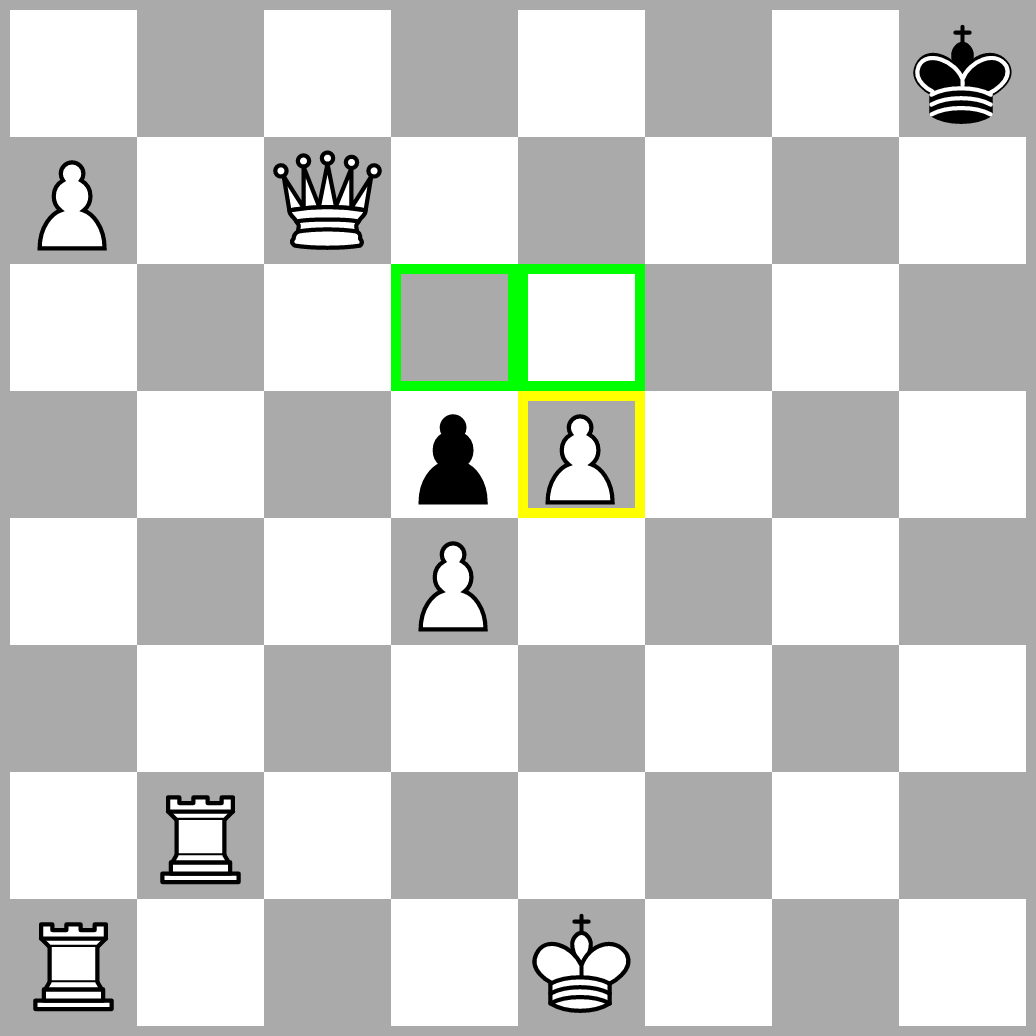
\includegraphics[width=.3\textwidth]{resources/evaluierung/chess/enpassant_before}
\caption{Evaluierung: En Passant vorher}
\label{fig:enpassant_before}
\end{figure}

\begin{figure}[h]
\centering
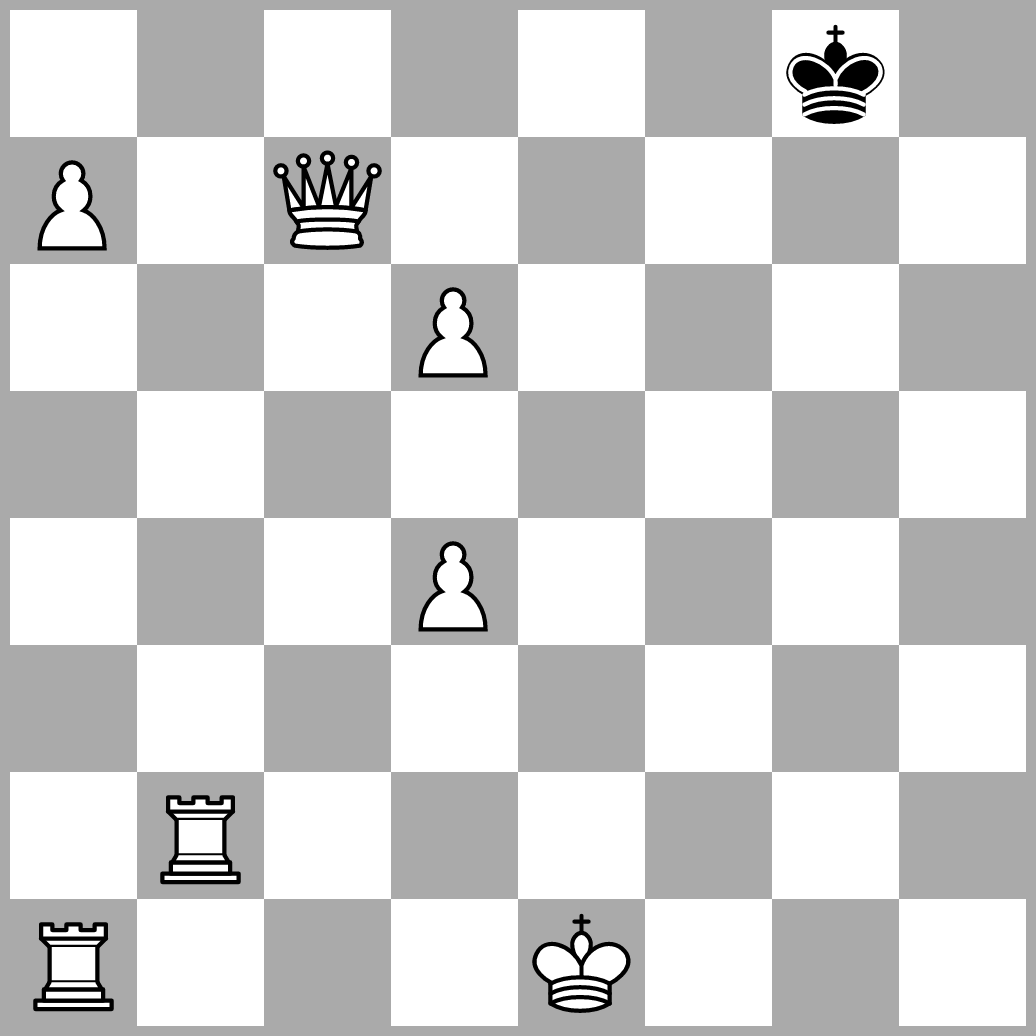
\includegraphics[width=.3\textwidth]{resources/evaluierung/chess/enpassant_after}
\caption{Evaluierung: En Passant danach}
\label{fig:enpassant_after}
\end{figure}

\begin{figure}[h]
\centering
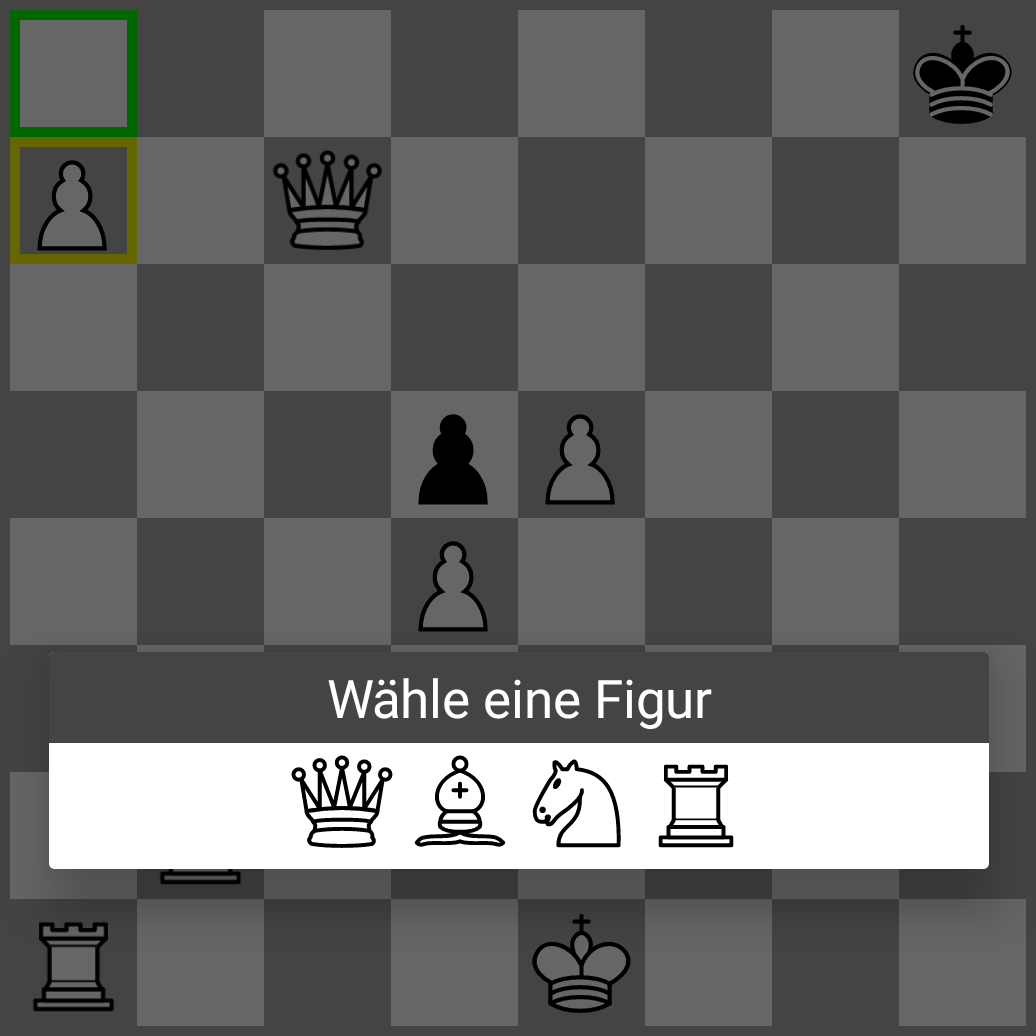
\includegraphics[width=.3\textwidth]{resources/evaluierung/chess/promotion_dialog}
\caption{Evaluierung: Promotionsdialog}
\label{fig:promotion_dialog}
\end{figure}

\begin{figure}[h]
\centering
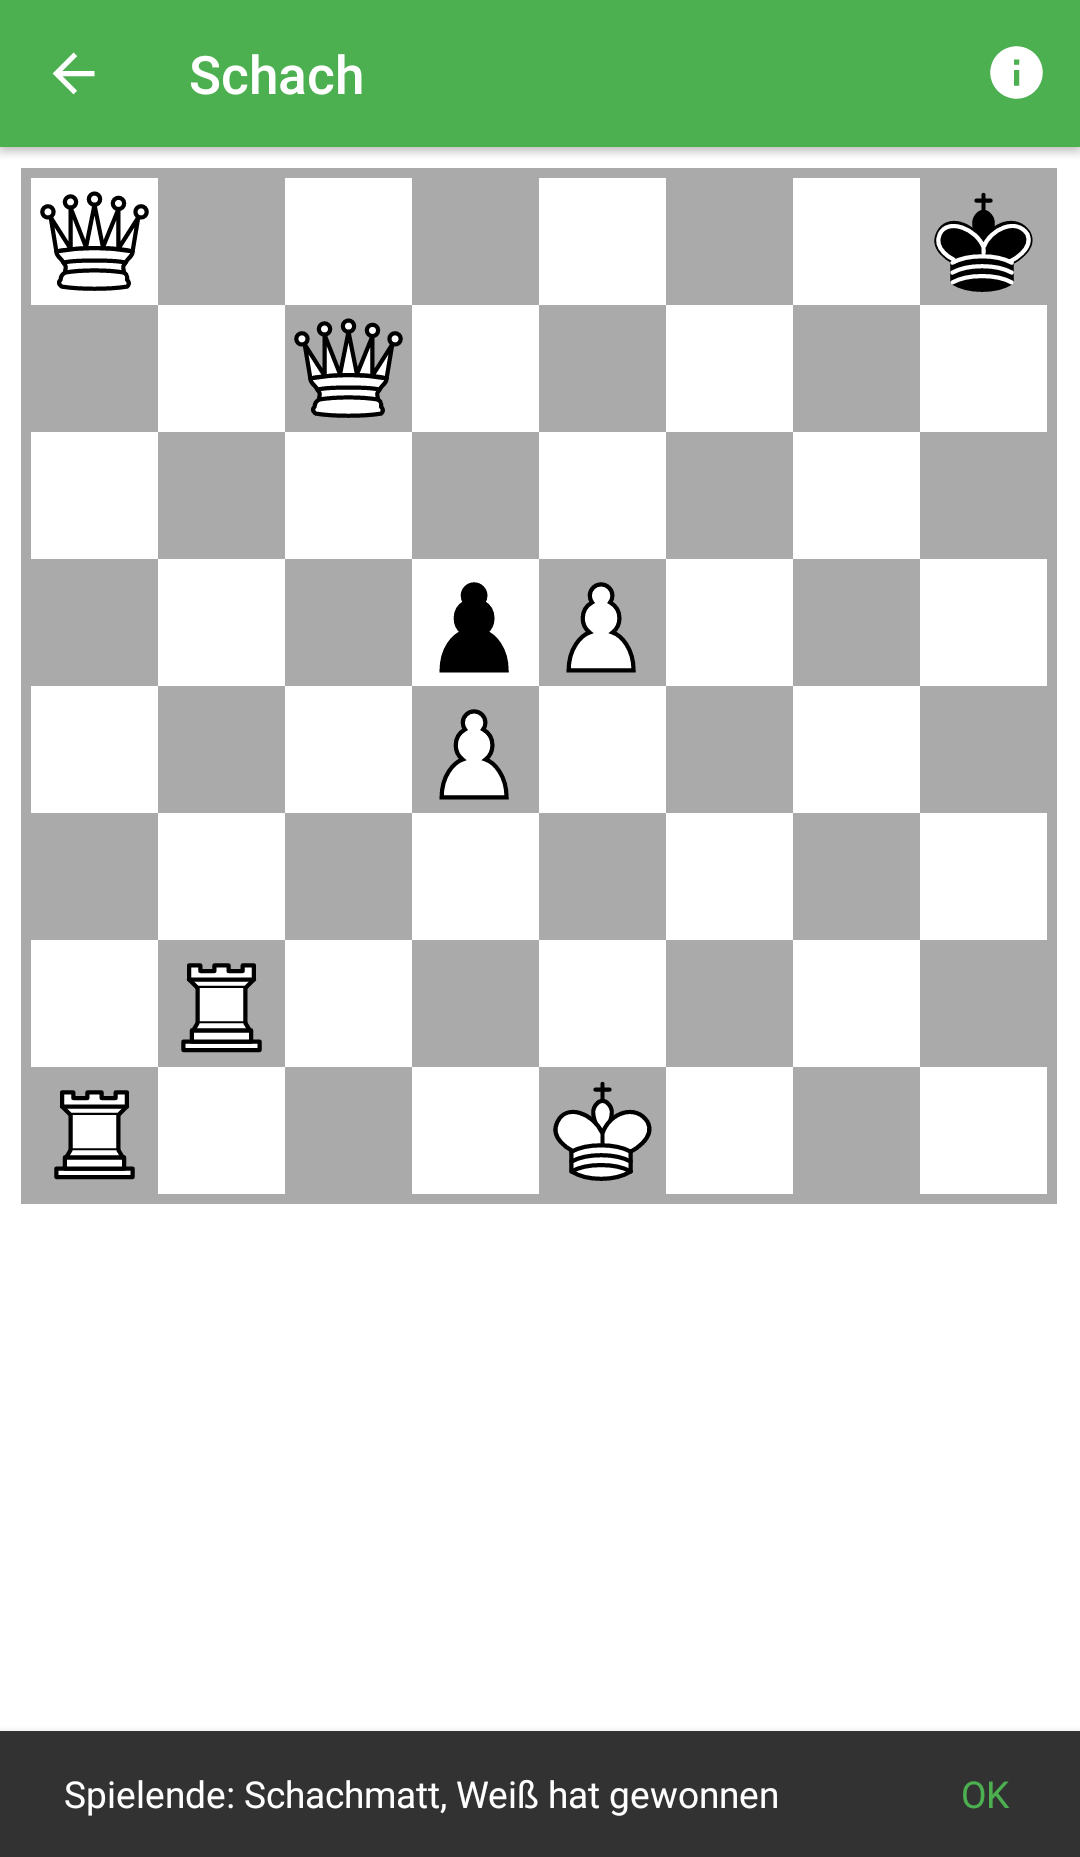
\includegraphics[width=.3\textwidth]{resources/evaluierung/chess/promotion_checkmate}
\caption{Evaluierung: Promotions-Schachmatt}
\label{fig:promotion_checkmate}
\end{figure}

\section{Kartenspielevaluierung}

\begin{figure}[h]
	\centering
	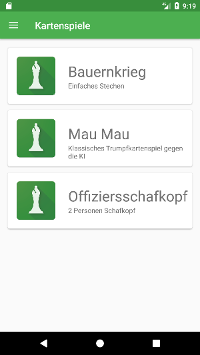
\includegraphics{resources/kartenscreens/auswahl}
	\caption{Auswahl der Spiele}
	\label{fig:cardgame_selection}
\end{figure}

\begin{figure}[h]
	\centering
	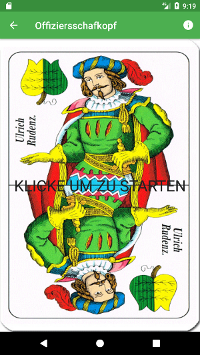
\includegraphics{resources/kartenscreens/menu}
	\caption{Spielmenu}
	\label{fig:cardgame_menu}
\end{figure}

\begin{figure}[h]
	\centering
	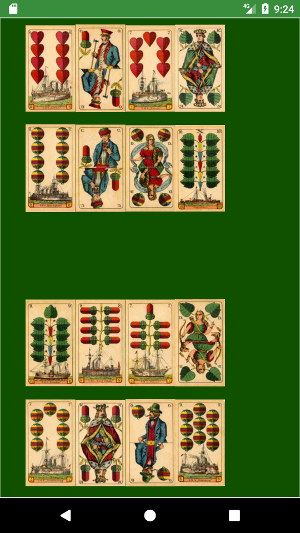
\includegraphics{resources/kartenscreens/board}
	\caption{Spielfeld Schafkopf}
	\label{fig:schafkopf}
\end{figure}

\begin{figure}[h]
	\centering
	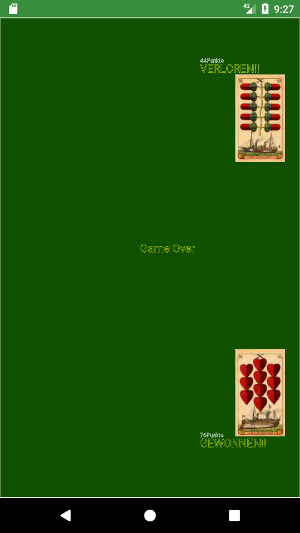
\includegraphics{resources/kartenscreens/gameover}
	\caption{Gameover Punkteanzeige}
	\label{fig:schafkopf_gameover}
\end{figure}
